\documentclass[a4paper,11pt]{article}

% ============================================================
%  Le Collé — Séance 1 : Déterminants, courbes paramétrées
%  © 2026 Ahmed Amine Ouqlani
% ============================================================

% ---------- Polices ----------
\usepackage[utf8]{inputenc}
\usepackage[T1]{fontenc}
\usepackage[sc]{mathpazo}          % texte et mathématiques : Palatino
\usepackage[scaled=0.88]{helvet}   % titres et repères : linéale
\linespread{1.07}
\usepackage{amsmath,amssymb,amsthm,mathrsfs,stmaryrd}
\usepackage{microtype}

% ---------- Mise en page ----------
\usepackage[a4paper,top=2.3cm,bottom=2.3cm,left=2.4cm,right=2.4cm,
            headheight=14pt,headsep=0.8cm,footskip=1.1cm]{geometry}
\setlength{\parindent}{0pt}
\setlength{\parskip}{0.45em plus 0.15em minus 0.1em}
\raggedbottom
\emergencystretch=1.5em
\clubpenalty=10000 \widowpenalty=10000 \displaywidowpenalty=10000 \brokenpenalty=10000

% ---------- Couleurs : un bleu de nuit, un ocre, des gris ----------
\usepackage{xcolor}
\definecolor{Ink}{HTML}{1C2533}
\definecolor{Bleu}{HTML}{1F3A5F}
\definecolor{BleuMoyen}{HTML}{4A6A8F}
\definecolor{BleuClair}{HTML}{9DB2C9}
\definecolor{Fond}{HTML}{F2F4F7}
\definecolor{Ocre}{HTML}{B07A26}
\definecolor{Brique}{HTML}{A23B2A}
\definecolor{Gris}{HTML}{5E6672}
\definecolor{Filet}{HTML}{C5CCD6}

% ---------- Packages ----------
\usepackage{enumitem}
\setlist{itemsep=0.25em,topsep=0.35em,parsep=0pt}
\setlist[itemize]{label=\textcolor{BleuMoyen}{\small\textbullet},leftmargin=1.4em}
\setlist[enumerate]{leftmargin=1.8em,label=\textsf{\small\color{Bleu}\arabic*.}}
\usepackage{booktabs,array,multicol}
\usepackage{needspace,float}
\usepackage[font=small,labelfont={sf,color=Bleu},labelsep=period,skip=6pt]{caption}
\usepackage{tikz}
\usetikzlibrary{arrows.meta,calc,decorations.markings}
\usepackage{pgfplots}
\pgfplotsset{compat=1.17}
\usepackage{tkz-tab}
\usepackage[most]{tcolorbox}
\usepackage{titlesec,titletoc}
\usepackage{fancyhdr,lastpage,etoolbox}
\usepackage[colorlinks=true,linkcolor=Bleu,urlcolor=Bleu,citecolor=Bleu,
            pdftitle={Le Collé — Propriétés métriques et enveloppes},pdfauthor={Ahmed Amine Ouqlani}]{hyperref}

\numberwithin{equation}{section}
\numberwithin{figure}{section}
\numberwithin{table}{section}

% ---------- Titres ----------
% Chapitres (sections) : grand numéro, titre en linéale, filet ocre
\titleformat{\section}[display]
  {\normalfont\sffamily\color{Ink}}
  {{\small\color{Gris}\textls[200]{\MakeUppercase{Chapitre}}}\\[-0.2em]%
   {\fontsize{64}{64}\selectfont\color{BleuClair}\thesection}}
  {0.4em}
  {\fontsize{25}{30}\selectfont\bfseries}
  [\vspace{0.5em}{\color{Ocre}\rule{3.2cm}{1.4pt}}]
\titlespacing*{\section}{0pt}{0pt}{1.6em}
\titleformat{name=\section,numberless}[display]
  {\normalfont\sffamily\color{Ink}}{}{0pt}{\fontsize{25}{30}\selectfont\bfseries}
  [\vspace{0.5em}{\color{Ocre}\rule{3.2cm}{1.4pt}}]
\titlespacing*{name=\section,numberless}{0pt}{0pt}{1.6em}

\titleformat{\subsection}
  {\needspace{5\baselineskip}\normalfont\sffamily\Large\bfseries\color{Ink}}
  {\color{Bleu}\thesubsection}{0.8em}{}
\titlespacing*{\subsection}{0pt}{1.8em}{0.5em}
\titleformat{\subsubsection}
  {\needspace{5\baselineskip}\normalfont\sffamily\large\bfseries\color{Ink}}
  {\color{Bleu}\thesubsubsection}{0.7em}{}
\titlespacing*{\subsubsection}{0pt}{1.6em}{0.4em}
\titleformat{\paragraph}[runin]{\normalfont\sffamily\bfseries\color{Ink}}{}{0pt}{}[.]
\titlespacing*{\paragraph}{0pt}{0.9em}{0.6em}
\setcounter{secnumdepth}{3}
\setcounter{tocdepth}{2}

% ---------- Table des matières ----------
\titlecontents{section}[0pt]{\addvspace{0.7em}\sffamily\bfseries\color{Ink}}
  {\makebox[2.2em][l]{\color{Bleu}\thecontentslabel}}{}{\hfill\contentspage}[\addvspace{0.2em}]
\titlecontents{subsection}[2.2em]{\small\linespread{1}\selectfont}
  {\makebox[2.6em][l]{\color{Gris}\thecontentslabel}}{}{\titlerule*[0.7pc]{.}\contentspage}

% ---------- En-têtes et pieds de page ----------
\pagestyle{fancy}
\fancyhf{}
\renewcommand{\sectionmark}[1]{\markboth{\thesection\quad#1}{}}
\fancyhead[L]{\footnotesize\sffamily\color{Gris}\leftmark}
\fancyhead[R]{\footnotesize\sffamily\scshape\color{Gris}Le Collé}
\fancyfoot[C]{\small\sffamily\color{Ink}\thepage}
\fancyfoot[L]{\scriptsize\sffamily\hyperlink{toc}{\color{Filet}sommaire}}
\renewcommand{\headrulewidth}{0.4pt}
\renewcommand{\headrule}{{\color{Filet}\hrule height\headrulewidth width\headwidth}}
\renewcommand{\footrulewidth}{0pt}
\fancypagestyle{plain}{\fancyhf{}\fancyfoot[C]{\small\sffamily\color{Ink}\thepage}\renewcommand{\headrulewidth}{0pt}}

% ---------- Énoncés ----------
\newtheoremstyle{enonce}{0pt}{0pt}{}{}{\sffamily\bfseries\color{Bleu}}{.}{0.5em}
  {\thmname{#1}\thmnumber{~#2}\thmnote{\ \normalfont\sffamily\color{Ink}(#3)}}
\newtheoremstyle{exemple}{0.9em}{0.9em}{}{}{\sffamily\bfseries\color{BleuMoyen}}{.}{0.5em}
  {\thmname{#1}\thmnumber{~#2}\thmnote{\ \normalfont\sffamily\color{Ink}(#3)}}
\newtheoremstyle{remarque}{0.7em}{0.7em}{}{}{\sffamily\itshape}{.}{0.5em}{\thmname{#1}\thmnote{\ (#3)}}
\theoremstyle{enonce}
\newtheorem{definition}{Définition}[section]
\newtheorem{theoreme}[definition]{Théorème}
\newtheorem{proposition}[definition]{Proposition}
\newtheorem{corollaire}[definition]{Corollaire}
\theoremstyle{exemple}
\newtheorem{exemple}[definition]{Exemple}
\theoremstyle{remarque}
\newtheorem*{remarque}{Remarque}

\tcbset{
  defi/.style={enhanced,breakable,colback=white,colframe=white,boxrule=0pt,arc=0pt,
     borderline west={1.2pt}{0pt}{Bleu},left=11pt,right=4pt,top=3pt,bottom=3pt,
     before skip=1.1em,after skip=1.1em},
  thm/.style={enhanced,breakable,colback=Fond,colframe=Fond,boxrule=0pt,arc=0pt,
     borderline west={2.4pt}{0pt}{Bleu},left=11pt,right=8pt,top=6pt,bottom=6pt,
     before skip=1.2em,after skip=1.2em}}
\tcolorboxenvironment{definition}{defi}
\tcolorboxenvironment{theoreme}{thm}
\tcolorboxenvironment{proposition}{thm}
\tcolorboxenvironment{corollaire}{thm}

\renewcommand{\proofname}{Démonstration}
\renewcommand{\qedsymbol}{\textcolor{BleuClair}{$\blacksquare$}}
\makeatletter
\renewenvironment{proof}[1][\proofname]{\par\pushQED{\qed}\normalfont
  \topsep0.5em\relax\trivlist\item[\hskip\labelsep\sffamily\itshape\color{Gris}#1.]\ignorespaces}
  {\popQED\endtrivlist\@endpefalse}
\makeatother

% ---------- Méthode : filets haut et bas, titre en bandeau ----------
\makeatletter\newcommand{\methlabelfix}{\protected@edef\@currentlabel{\thetcbcounter}}\makeatother
\newtcolorbox[auto counter,number within=section]{methode}[2][]{%
  enhanced,unbreakable,colback=white,colframe=white,boxrule=0pt,arc=0pt,
  borderline north={0.9pt}{0pt}{Bleu},borderline south={0.9pt}{0pt}{Bleu},
  left=4pt,right=4pt,top=8pt,bottom=8pt,before skip=1.4em,after skip=1.4em,
  before upper={\methlabelfix\phantomsection\addcontentsline{met}{metentry}{\protect\makebox[2.6em][l]{\thetcbcounter}#2}%
     {\sffamily\bfseries\small\color{white}\colorbox{Bleu}{\strut\ MÉTHODE~\thetcbcounter\ }}%
     \ \ {\sffamily\bfseries\color{Bleu}#2}\par\smallskip},#1}

% ---------- Repères pédagogiques : un filet de couleur, un mot-clé ----------
\newcommand{\definirbloc}[3]{% nom, couleur, libellé
  \newtcolorbox{#1}[1][]{enhanced,breakable,blanker,
    borderline west={1.4pt}{0pt}{#2},left=10pt,right=2pt,top=1pt,bottom=1pt,
    before skip=1em,after skip=1em,
    before upper={{\sffamily\bfseries\footnotesize\color{#2}\textls[120]{\MakeUppercase{#3}}}\quad},##1}}
\definirbloc{reflexe}{Bleu}{Réflexe}
\definirbloc{astuce}{Ocre}{Astuce}
\definirbloc{attention}{Brique}{Attention}
\definirbloc{enpratique}{BleuMoyen}{En pratique}
\definirbloc{plusloin}{Gris}{Pour aller plus loin}
\definirbloc{strategie}{Bleu}{Stratégie}
\definirbloc{lecture}{BleuMoyen}{Lire le schéma}
% compatibilité avec les parties reprises
\newenvironment{garde}{\begin{attention}}{\end{attention}}
\newenvironment{complementHP}{\begin{plusloin}}{\end{plusloin}}
\newenvironment{interpretation}{\begin{enpratique}}{\end{enpratique}}

% ---------- Exercices, corrigés ----------
\newcounter{exo}[section]
\renewcommand{\theexo}{\thesection.\arabic{exo}}
\newcommand{\niveau}[1]{{\color{Ocre}\footnotesize
  \ifcase#1\or$\bullet\circ\circ\circ\circ$\or$\bullet\bullet\circ\circ\circ$\or$\bullet\bullet\bullet\circ\circ$%
  \or$\bullet\bullet\bullet\bullet\circ$\or$\bullet\bullet\bullet\bullet\bullet$\fi}}
\newcommand{\serie}[1]{\par\needspace{8\baselineskip}\vspace{1.5em}%
  \noindent{\sffamily\bfseries\color{Bleu}#1}\par\nobreak\vspace{-0.4em}%
  \noindent{\color{Filet}\rule{\linewidth}{0.4pt}}\par\nobreak\vspace{0.1em}}
\newenvironment{exo}[3]{%
  \par\needspace{5\baselineskip}\vspace{0.75em}\refstepcounter{exo}\label{e:#1}%
  \def\exolab{#1}%
  \noindent{\sffamily\bfseries\color{Bleu}Exercice~\theexo}\quad\niveau{#2}%
  \hfill{\footnotesize\sffamily\color{Gris}#3}\par\nobreak\vspace{0.15em}}%
  {\par\nopagebreak\noindent\hfill{\scriptsize\sffamily\hyperref[c:\exolab]{\color{Gris}corrigé p.~\pageref{c:\exolab}}}\par}
\newenvironment{corrige}[1]{%
  \par\needspace{6\baselineskip}\vspace{1em}\phantomsection\label{c:#1}%
  \noindent{\sffamily\bfseries\color{Bleu}Exercice~\ref{e:#1}}\quad
  {\scriptsize\sffamily\hyperref[e:#1]{\color{Gris}énoncé p.~\pageref{e:#1}}}\par\nobreak\vspace{0.2em}}%
  {\hfill\textcolor{BleuClair}{$\square$}\par}
\newcommand{\etape}[1]{\par\smallskip\noindent{\sffamily\bfseries\small\color{BleuMoyen}#1.}\ }
\newenvironment{solution}{\par\noindent{\sffamily\bfseries\small\color{BleuMoyen}Solution.}\ }{\hfill\textcolor{BleuClair}{$\square$}\par}
\newcommand{\chercher}{\par\smallskip\noindent{\color{Filet}\rule[0.5ex]{1.2cm}{0.4pt}}\
  {\footnotesize\sffamily\itshape\color{Gris}laisser chercher l'étudiant avant de poursuivre}\par\smallskip}

% ---------- Guide de séance ----------

\newcommand{\marge}[1]{\leavevmode\marginpar{\raggedleft\scriptsize\sffamily\color{Gris}\textls[100]{\MakeUppercase{#1}}}\ignorespaces}
\newcommand{\Etape}[4]{%
  \subsection[Étape #1 --- #3 {\color{Gris}(#2)}]{#3}\label{etape:#1}%
  \noindent{\small\sffamily\color{Gris}{\color{Ocre}\bfseries Étape #1}\quad·\quad #2\quad·\quad #4}\par\medskip}
\newcommand{\question}[1]{\par\smallskip\noindent{\sffamily\bfseries\small\color{BleuMoyen}Question.}\ \textit{#1}\par\smallskip}
\newcommand{\rappel}[1]{\par\smallskip\noindent\phantomsection\addcontentsline{rap}{rapentry}{#1}%
  {\sffamily\bfseries\scriptsize\colorbox{Fond}{\color{Gris}\strut RAPPEL}}\ {\sffamily\small\color{Gris}#1.}\ }
\newcommand{\pourquoi}{\par\noindent{\sffamily\bfseries\small\color{Ocre}Pourquoi ?}\ }

% Ouverture de chapitre : \ouverture{objectifs}{prérequis}{durée}
\newcommand{\ouverture}[3]{%
  \begin{tcolorbox}[enhanced,colback=Fond,colframe=Fond,arc=0pt,boxrule=0pt,left=12pt,right=12pt,top=10pt,bottom=10pt,
     before skip=1.2em,after skip=1.6em]
  \begin{minipage}[t]{0.56\linewidth}
  {\sffamily\bfseries\small\color{Bleu}OBJECTIFS}\par\vspace{0.3em}\small #1
  \end{minipage}\hfill
  \begin{minipage}[t]{0.38\linewidth}
  {\sffamily\bfseries\small\color{Bleu}PRÉREQUIS}\par\vspace{0.3em}\small #2
  \ifx\relax#3\relax\else\par\vspace{0.6em}{\sffamily\bfseries\small\color{Bleu}DURÉE}\par\vspace{0.2em}\small #3\fi
  \end{minipage}
  \end{tcolorbox}}
% Fin de chapitre
\newenvironment{essentiel}{\par\needspace{12\baselineskip}\vspace{1.5em}%
  \begin{tcolorbox}[enhanced,unbreakable,colback=white,colframe=white,boxrule=0pt,arc=0pt,
   borderline north={1.4pt}{0pt}{Ocre},left=2pt,right=2pt,top=8pt,bottom=4pt]
  {\sffamily\bfseries\color{Ocre}L'ESSENTIEL DU CHAPITRE}\par\medskip}{\end{tcolorbox}}

% ---------- Notations ----------
\newcommand{\K}{\mathbb{K}}
\newcommand{\R}{\mathbb{R}}
\newcommand{\C}{\mathbb{C}}
\newcommand{\N}{\mathbb{N}}
\newcommand{\Z}{\mathbb{Z}}
\newcommand{\Mn}[1]{\mathcal{M}_{n}(#1)}
\newcommand{\GLn}[1]{\mathrm{GL}_n(#1)}
\newcommand{\LE}{\mathcal{L}(E)}
\newcommand{\rg}{\operatorname{rg}}
\newcommand{\vect}{\operatorname{Vect}}
\newcommand{\Mat}{\operatorname{Mat}}
\newcommand{\Id}{\operatorname{Id}}
\newcommand{\sh}{\operatorname{sh}}
\newcommand{\ch}{\operatorname{ch}}
\renewcommand{\th}{\operatorname{th}}
\DeclareMathOperator{\argsh}{argsh}
\newcommand{\vv}[1]{\overrightarrow{#1}}
\newcommand{\ve}[1]{\vec{#1}}
\newcommand{\ient}[2]{\llbracket #1,#2\rrbracket}
\newcommand{\dt}[1]{\left|\begin{matrix}#1\end{matrix}\right|}
\newcommand{\dis}{\displaystyle}

% ---------- Figures ----------
\pgfplotsset{trig format plots=rad}
\pgfplotsset{courbe/.style={axis lines=middle,axis equal image,
  axis line style={Gris,-{Stealth[length=5pt]}},
  xlabel={$x$},ylabel={$y$},ticklabel style={font=\scriptsize\sffamily,color=Gris},
  every axis x label/.style={at={(ticklabel* cs:1)},anchor=west,font=\small},
  every axis y label/.style={at={(ticklabel* cs:1)},anchor=south,font=\small},
  samples=300,smooth,width=0.6\linewidth}}
\tikzset{arcetude/.style={Bleu,line width=1.25pt},
         reste/.style={BleuClair,line width=1pt},
         tgte/.style={Ocre,line width=0.9pt},
         asy/.style={Gris,dashed,line width=0.6pt},
         pt/.style={circle,fill=Ink,inner sep=1.2pt}}

% ---------- Navigation ----------
\makeatletter
\newcommand*\l@rapentry{\@dottedtocline{1}{0em}{0em}}
\newcommand*\l@metentry{\@dottedtocline{1}{0em}{0em}}
\newcommand{\listemethodes}{\@starttoc{met}}
\newcommand{\listerappels}{\@starttoc{rap}}
\makeatother
% onglets de chapitre sur le bord droit
\usepackage{eso-pic}
\newif\ifonglets \ongletsfalse
\newcommand{\dessineronglet}{%
  \edef\ongcol{\ifnum\value{section}=3 Ocre\else Bleu\fi}%
  \edef\ongnum{\the\value{section}}%
  \pgfmathsetmacro{\ongy}{3.2+2.3*(\ongnum-1)}%
  \begin{tikzpicture}[remember picture,overlay]
  \fill[\ongcol] ([xshift=-0.75cm,yshift=-\ongy cm]current page.north east)
     rectangle ([yshift=-\ongy cm-1.9cm]current page.north east);
  \node[text=white,font=\sffamily\bfseries\large] at ([xshift=-0.37cm,yshift=-\ongy cm-0.95cm]current page.north east)
     {\ongnum};
  \end{tikzpicture}}
\AddToShipoutPictureBG{\ifonglets\ifnum\value{section}>0 \dessineronglet\fi\fi}
% blocs de navigation et d'enseignement
\definirbloc{commencer}{Gris}{Si vous commencez ici}
\definirbloc{horsprogramme}{Brique}{Hors programme}
\newcommand{\HP}{\,{\sffamily\bfseries\scriptsize\textcolor{Brique}{[HP]}}}
\newcommand{\source}[1]{{\footnotesize\sffamily\color{Gris}\,(#1)}}
\newcommand{\coupdepouce}[1]{\par\vspace{-0.2em}\noindent{\footnotesize\sffamily\color{Gris}%
  \textbf{Coup de pouce} (à donner si l'étudiant bloque) : #1}\par}
\newcommand{\pointarret}[1]{\par\vspace{1em}\noindent{\color{Filet}\rule[0.5ex]{\linewidth}{0.4pt}}\par\nobreak
  \noindent{\footnotesize\sffamily\color{Ocre}\bfseries POINT D'ARRÊT POSSIBLE}\quad{\footnotesize\sffamily\color{Gris}#1}\par\vspace{0.6em}}
\newcommand{\demarche}[1]{\noindent{\sffamily\bfseries\small\color{BleuMoyen}Démarche.}\ \textit{#1}\par\smallskip}

% ---------- Corrigés : idées, astuces, pièges, à retenir ----------
\newcommand{\choix}[1]{\par\noindent{\sffamily\bfseries\small\color{BleuMoyen}Choix de la méthode.}\ #1\par\smallskip}
\newcommand{\gain}[1]{\par\noindent{\sffamily\bfseries\small\color{Ocre}Astuce.}\ #1\par}
\newcommand{\piege}[1]{\par\noindent{\sffamily\bfseries\small\color{Brique}Piège.}\ #1\par}
\newtcolorbox{retenirbox}{enhanced,breakable,colback=Fond,colframe=Fond,arc=0pt,boxrule=0pt,
  borderline west={2pt}{0pt}{Ocre},left=8pt,right=6pt,top=4pt,bottom=4pt,before skip=0.7em,after skip=0.5em}
\newcommand{\retenir}[1]{\begin{retenirbox}{\sffamily\bfseries\footnotesize\color{Ocre}À RETENIR}\quad #1\end{retenirbox}}
\newcommand{\TD}[1]{{\color{Ocre}\bfseries TD\,#1}\ ·\ }
\newcommand{\q}[1]{\par\smallskip\noindent{\sffamily\bfseries\color{Bleu}#1}\ }
\providecommand{\iddots}{\mathinner{\mkern1mu\raise1pt\hbox{.}\mkern2mu\raise4pt\hbox{.}\mkern2mu\raise7pt\hbox{.}\mkern1mu}}

\begin{document}
\pagenumbering{roman}

% ======================= Couverture =======================
\begin{titlepage}
\thispagestyle{empty}
\begin{tikzpicture}[remember picture,overlay]
  % bandeau supérieur
  \fill[Bleu] (current page.north west) rectangle ([yshift=-15.5cm]current page.north east);
  % motif : quelques arches de cycloïde et une cardioïde, en filigrane
  \begin{scope}[shift={([xshift=-1.2cm,yshift=-15.5cm]current page.north west)},x=1.05cm,y=1.05cm]
    \draw[BleuMoyen,line width=0.7pt,domain=0:25.2,samples=400,smooth]
      plot ({\x-sin(\x r)},{1-cos(\x r)});
  \end{scope}
  \begin{scope}[shift={([xshift=-3.6cm,yshift=-11.2cm]current page.north east)},scale=0.75]
    \draw[BleuMoyen,line width=0.6pt,domain=0:6.2832,samples=300,smooth]
      plot ({2*cos(\x r)-cos(2*\x r)},{2*sin(\x r)-sin(2*\x r)});
  \end{scope}
  % titre
  \node[anchor=north west,text=white,font=\sffamily\small] at ([xshift=2.6cm,yshift=-3.2cm]current page.north west)
     {\textls[250]{MATHÉMATIQUES\ \ ·\ \ CPGE PT\ \ ·\ \ DEUXIÈME ANNÉE}};
  \node[anchor=north west,text=white] at ([xshift=2.5cm,yshift=-4.4cm]current page.north west)
     {\fontsize{62}{66}\selectfont\scshape Le Collé};
  \draw[Ocre,line width=1.6pt] ([xshift=2.6cm,yshift=-7.3cm]current page.north west) -- ++(4.2cm,0);
  \node[anchor=north west,text=white,font=\sffamily\Large\bfseries,align=left]
     at ([xshift=2.6cm,yshift=-8.0cm]current page.north west)
     {Propriétés métriques et enveloppes};
  \node[anchor=north west,text=white!90!Bleu,font=\sffamily\large,align=left]
     at ([xshift=2.6cm,yshift=-9.0cm]current page.north west)
     {Longueur, courbure, développée\\[0.15cm]Enveloppe d'une famille de droites};
  % bas de page
  \node[anchor=north west,text=Ink,font=\sffamily\small,align=left,text width=12cm]
     at ([xshift=2.6cm,yshift=-17.4cm]current page.north west)
     {\textcolor{Bleu}{\bfseries Cours, méthodes et exercices corrigés}\\[0.3cm]
      \textcolor{Gris}{Le complément métrique du volume \emph{Déterminants, courbes paramétrées planes} :
      cours, méthodes et exercices corrigés.}};
  \node[anchor=south west,text=Ink,font=\sffamily\large] at ([xshift=2.6cm,yshift=3.0cm]current page.south west)
     {Ahmed Amine Ouqlani};
  \draw[Filet] ([xshift=2.6cm,yshift=2.6cm]current page.south west) -- ([xshift=-2.4cm,yshift=2.6cm]current page.south east);
\end{tikzpicture}
\end{titlepage}

\thispagestyle{plain}
\section*{Avant-propos}
\markboth{Avant-propos}{}

Ce volume complète \emph{Déterminants, courbes paramétrées planes} et en reprend la forme. Il couvre la fin du programme de PT
sur les courbes : longueur et abscisse curviligne, repère de Frenet, courbure, rayon, centre et cercle de courbure, développée,
enveloppe d'une famille de droites. Le programme privilégie la vision géométrique : chaque formule est donc accompagnée de
son origine et de son interprétation, et les questions de régularité ne sont pas soulevées. Les notations ($f(t)=\vv{OM(t)}$,
point régulier, birégulier, $\det(f',f'')$) sont celles du premier volume. Les corrigés, regroupés au chapitre~3, indiquent le
choix de la méthode, les astuces, les pièges et ce qu'il faut retenir.

\vfill
{\footnotesize\sffamily\color{Gris}\textcopyright~2026 Ahmed Amine Ouqlani. Tous droits réservés.\par}

\clearpage
\thispagestyle{plain}
\hypertarget{toc}{}
\renewcommand{\contentsname}{Sommaire}
\tableofcontents
\clearpage
\pagenumbering{arabic}
\ongletstrue
% =====================================================================
%            CHAPITRE 1 — PROPRIÉTÉS MÉTRIQUES DES COURBES PLANES
% =====================================================================
\clearpage
\section{Propriétés métriques des courbes planes}

L'étude du premier volume décrit l'\emph{allure} d'une courbe. Les propriétés métriques la \emph{mesurent} : combien elle est
longue, à quelle vitesse sa tangente tourne, quel cercle l'épouse le mieux en un point. Toutes se ramènent à une idée :
reparamétrer la courbe par la distance parcourue.

% ---------------------------------------------------------------------
\subsection{Longueur et abscisse curviligne}

Pendant la durée $dt$, le point parcourt environ $\|f'(t)\|\,dt$ (vitesse fois durée) ; en sommant, on obtient la longueur.

\begin{definition}
La \emph{longueur} de l'arc $t\in[a,b]$ d'une courbe régulière est $L=\int_a^b\|f'(t)\|\,dt=\int_a^b\sqrt{x'(t)^2+y'(t)^2}\,dt$.
Une \emph{abscisse curviligne} est une fonction $s$ telle que $s'(t)=\|f'(t)\|$, par exemple $s(t)=\int_{t_0}^t\|f'(u)\|\,du$ :
c'est la longueur parcourue depuis $M(t_0)$, comptée positivement dans le sens des $t$ croissants.
\end{definition}

La définition est celle du programme ; géométriquement, $L$ est la limite des longueurs des lignes polygonales inscrites.
Elle ne dépend pas du paramétrage : si $t=\varphi(u)$ avec $\varphi$ croissante, $\|(f\circ\varphi)'(u)\|\,du=\|f'(t)\|\,dt$. Comme
$s$ est strictement croissante (courbe régulière), on peut paramétrer par $s$ : c'est le \emph{paramétrage normal}, de vitesse
$1$, et $\frac{dM}{ds}=\frac{f'(t)}{\|f'(t)\|}$.

\begin{attention}
$L$ mesure une distance \emph{parcourue} : une portion décrite deux fois compte deux fois. On intègre sur un intervalle où
chaque arc est décrit une seule fois, en exploitant les symétries (longueur totale $=$ nombre d'arcs $\times$ longueur d'un
arc). Ne pas oublier la valeur absolue dans $\|f'\|=\sqrt{\dots}$ : $\sqrt{4\sin^2\frac t2}=2\left|\sin\frac t2\right|$.
\end{attention}

\begin{exemple}[la cardioïde]
Pour $f(t)=\big((1-\cos t)\cos t,(1-\cos t)\sin t\big)$, $x'^2+y'^2=2-2\cos t=4\sin^2\frac t2$, donc
$L=\int_0^{2\pi}2\sin\frac t2\,dt=\left[-4\cos\frac t2\right]_0^{2\pi}=8$ (sur $[0,4\pi]$, on trouverait $16$ pour la même courbe).
\end{exemple}

\begin{exo}{m-cycl}{2}{longueur, abscisse curviligne}
Soit la cycloïde $f(t)=(t-\sin t,\ 1-\cos t)$.
\begin{enumerate}
\item Calculer la longueur d'une arche, $t\in[0,2\pi]$.
\item Déterminer l'abscisse curviligne $s$ d'origine $O=M(0)$, orientée dans le sens des $t$ croissants.
\end{enumerate}
\end{exo}
\begin{exo}{m-astro}{3}{longueur totale, symétries}
Calculer la longueur totale de l'astroïde $f(t)=(\cos^3t,\sin^3t)$, $t\in[0,2\pi]$.
\end{exo}

% ---------------------------------------------------------------------
\subsection{Repère de Frenet et courbure}

\begin{definition}
En un point régulier d'une courbe orientée, le \emph{vecteur unitaire tangent} est $\ve T=\frac{dM}{ds}=\frac{f'}{\|f'\|}$, et le
\emph{vecteur normal} $\ve N$ s'en déduit par rotation de $+\frac\pi2$ : si $\ve T=(a,b)$, $\ve N=(-b,a)$. $(M,\ve T,\ve N)$ est le
\emph{repère de Frenet}. On écrit $\ve T=\cos\alpha\,\ve\imath+\sin\alpha\,\ve\jmath$, où $\alpha$ est l'angle de la tangente
avec l'axe $(Ox)$.
\end{definition}

\begin{definition}
Comme $\|\ve T\|=1$, $\frac{d\ve T}{ds}$ est orthogonal à $\ve T$ (dériver $\ve T\cdot\ve T=1$) : il existe un réel $\gamma$, la
\emph{courbure}, tel que
\[\frac{d\ve T}{ds}=\gamma\,\ve N,\qquad\text{et alors}\qquad\frac{d\ve N}{ds}=-\gamma\,\ve T\quad\text{(formules de Frenet)}.\]
\end{definition}

\begin{proposition}\label{prop:alpha}
$\gamma=\dfrac{d\alpha}{ds}$ : la courbure est la vitesse de rotation de la tangente, par unité de longueur parcourue.
\end{proposition}

\begin{proof}
$\ve T=(\cos\alpha,\sin\alpha)$ donne $\frac{d\ve T}{ds}=\frac{d\alpha}{ds}(-\sin\alpha,\cos\alpha)=\frac{d\alpha}{ds}\ve N$. De même
$\ve N=(-\sin\alpha,\cos\alpha)$ donne $\frac{d\ve N}{ds}=-\frac{d\alpha}{ds}\ve T$.
\end{proof}

\paragraph{Interprétation} $|\gamma|$ mesure à quel point la courbe tourne : nulle sur une droite, constante égale à
$\frac1R$ sur un cercle de rayon $R$ (parcouru dans le sens direct, $\alpha=\frac sR+\text{cte}$). Le \emph{signe} de $\gamma$
dit de quel côté elle tourne : $\gamma>0$, la tangente tourne dans le sens direct et la courbe s'incurve du côté de $\ve N$
(vers la gauche quand on la parcourt) ; $\gamma<0$, vers la droite.

\begin{horsprogramme}
\textbf{Courbure et déterminant.} Avec $v=\frac{ds}{dt}=\|f'\|$ : $f'=v\ve T$, puis
$f''=v'\ve T+v\frac{d\ve T}{dt}=v'\ve T+v^2\gamma\ve N$ ; donc $\det(f',f'')=v^3\gamma\det(\ve T,\ve N)=v^3\gamma$, et
\[\gamma=\frac{\det\big(f'(t),f''(t)\big)}{\|f'(t)\|^3}.\]
C'est l'origine du rôle de $\det(f',f'')$ dans le premier volume : un point est \emph{birégulier} si et seulement si $\gamma\neq0$,
et une inflexion est un point où $\gamma$ change de signe. La formule est hors programme mais très utile pour vérifier un
calcul ; le programme préfère $\gamma=\frac{d\alpha}{ds}$.
\end{horsprogramme}

\begin{methode}{Calculer une courbure}\label{meth:courbure}
\begin{enumerate}
\item Calculer $f'$ et l'écrire $f'(t)=v(t)\,(\cos\alpha(t),\sin\alpha(t))$ avec $v>0$ : on lit $\frac{ds}{dt}=v$ et l'angle $\alpha$
      (factoriser par l'angle moitié si besoin).
\item $\gamma=\frac{d\alpha}{ds}=\frac{\alpha'(t)}{v(t)}$.
\item Contrôle : $\gamma=\frac{\det(f',f'')}{v^3}$.
\end{enumerate}
\end{methode}

% ---------------------------------------------------------------------
\subsection{Rayon, centre et cercle de courbure ; développée}

\begin{definition}
En un point birégulier ($\gamma\neq0$), le \emph{rayon de courbure} est $R=\frac1\gamma$ (algébrique), le \emph{centre de
courbure} est $I=M+R\,\ve N$, et le \emph{cercle de courbure} (ou osculateur) est le cercle de centre $I$ et de rayon $|R|$.
La \emph{développée} d'une courbe birégulière est l'ensemble de ses centres de courbure.
\end{definition}

\paragraph{Interprétation} Le cercle de courbure est tangent à la courbe en $M$, situé du côté vers lequel elle s'incurve,
et il a la même courbure : c'est le cercle qui épouse le mieux la courbe en $M$. Plus la courbe est « plate », plus $|R|$ est
grand ; en une inflexion, $R$ devient infini.

\begin{figure}[H]
\centering
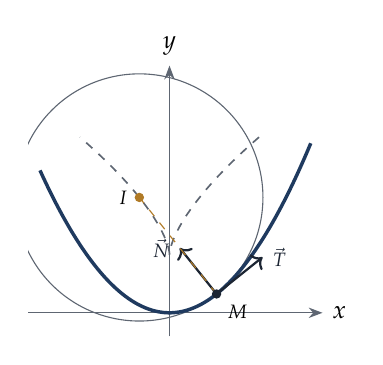
\begin{tikzpicture}
\begin{axis}[courbe,width=0.48\linewidth,xmin=-2.4,xmax=2.6,ymin=-0.4,ymax=4.2,xtick=\empty,ytick=\empty]
\addplot[asy,domain=-1.15:1.15,samples=80]({-x^3},{1+1.5*x^2});
\addplot[Gris,thin,domain=0:6.2832,samples=150]({-0.512+2.1*cos(x)},{1.96+2.1*sin(x)});
\addplot[arcetude,domain=-2.2:2.4,samples=100]{x^2/2};
\draw[->,thick,Ink] (axis cs:0.8,0.32)--(axis cs:1.581,0.945) node[right,font=\scriptsize]{$\ve T$};
\draw[->,thick,Ink] (axis cs:0.8,0.32)--(axis cs:0.175,1.101) node[left,font=\scriptsize]{$\ve N$};
\draw[Ocre,dashed] (axis cs:0.8,0.32)--(axis cs:-0.512,1.96);
\node[pt] at (axis cs:0.8,0.32) {}; \node[font=\scriptsize,anchor=north west] at (axis cs:0.82,0.3) {$M$};
\node[pt,fill=Ocre] at (axis cs:-0.512,1.96) {}; \node[font=\scriptsize,anchor=east] at (axis cs:-0.55,1.96) {$I$};
\end{axis}
\end{tikzpicture}
\caption{La parabole $y=\frac{x^2}2$, le repère de Frenet en $M$, le cercle de courbure (gris) de centre $I$, et la développée
(pointillés), lieu des centres de courbure.}\label{fig:frenet}
\end{figure}

\begin{exemple}[développée de la parabole]
$f(t)=\left(t,\frac{t^2}2\right)$ : $f'=(1,t)$, $v=\sqrt{1+t^2}$, $\ve N=\frac{(-t,1)}{\sqrt{1+t^2}}$, et
$\gamma=\frac{\det(f',f'')}{v^3}=\frac1{(1+t^2)^{3/2}}$. Donc $R=(1+t^2)^{3/2}$ et
\[I=M+R\ve N=\left(t,\tfrac{t^2}2\right)+(1+t^2)(-t,1)=\left(-t^3,\ 1+\tfrac32t^2\right) :\]
la développée est une parabole semi-cubique, qui présente un rebroussement en $(0,1)$, centre de courbure au sommet ($R=1$).
\end{exemple}

\begin{reflexe}
Aux points d'une courbe situés sur un axe de symétrie, la courbure est stationnaire (souvent extrémale : ce sont les
\emph{sommets}) et le centre de courbure est sur l'axe : la développée y présente en général un rebroussement.
\end{reflexe}

\begin{exo}{m-ellipse}{3}{courbure, rayon de courbure aux sommets}
Soit l'ellipse $f(t)=(a\cos t,b\sin t)$, $a>b>0$.
\begin{enumerate}
\item Montrer que $\alpha'(t)=\frac{\det(f',f'')}{\|f'\|^2}$ (où $\alpha$ est l'angle de la tangente), puis calculer la courbure.
\item Calculer le rayon de courbure aux quatre sommets. Où la courbure est-elle maximale ?
\end{enumerate}
\end{exo}
\begin{exo}{m-cycl-dev}{4}{repère de Frenet, centre de courbure, développée}
On reprend la cycloïde $f(t)=(t-\sin t,1-\cos t)$, $t\in\,]0,2\pi[$.
\begin{enumerate}
\item Déterminer $\ve T$, $\ve N$, l'angle $\alpha$ et la courbure $\gamma$.
\item Montrer que le centre de courbure est $I(t)=(t+\sin t,\ \cos t-1)$.
\item En déduire que la développée de la cycloïde est une cycloïde, image de la première par une translation.
\end{enumerate}
\end{exo}
% =====================================================================
%            CHAPITRE 2 — ENVELOPPE D'UNE FAMILLE DE DROITES
% =====================================================================
\clearpage
\section{Enveloppe d'une famille de droites}

Une famille de droites peut « dessiner » une courbe sans qu'on la trace : la courbe à laquelle chacune est tangente. C'est
l'\emph{enveloppe}. Le programme privilégie la vision géométrique : deux droites voisines de la famille se coupent sur
l'enveloppe.

% ---------------------------------------------------------------------
\subsection{Définition et calcul}\label{sec:enveloppe}

\begin{definition}
Soit une famille de droites $\mathcal D_t=A(t)+\vect\big(\ve u(t)\big)$, $A$ et $\ve u$ de classe $\mathcal C^1$, $\ve u(t)\neq\ve0$.
On cherche $\lambda$ de classe $\mathcal C^1$ telle que $M(t)=A(t)+\lambda(t)\ve u(t)$ paramètre une courbe dont la tangente en
$M(t)$ est dirigée par $\ve u(t)$ : le point $M(t)$ est sur $\mathcal D_t$, et $\mathcal D_t$ y est tangente. La courbe décrite
par $M$ est l'enveloppe ; $M(t)$ est le \emph{point caractéristique} de $\mathcal D_t$.
\end{definition}

\emph{Comment trouver $\lambda$.} $M'=A'+\lambda'\ve u+\lambda\ve u'$ doit être colinéaire à $\ve u$ : comme $\det(\ve u,\ve u)=0$,
la condition $\det(M',\ve u)=0$ s'écrit $\det(A',\ve u)+\lambda\det(\ve u',\ve u)=0$, d'où, si $\det(\ve u,\ve u')\neq0$,
\[\lambda(t)=\frac{\det\big(A'(t),\ve u(t)\big)}{\det\big(\ve u(t),\ve u'(t)\big)}.\]
\emph{Vision géométrique} : $M(t)$ est la position limite de l'intersection de $\mathcal D_t$ et de $\mathcal D_{t+h}$ quand
$h\to0$ (deux droites infiniment voisines se coupent sur l'enveloppe).

\begin{methode}{Calculer une enveloppe}\label{meth:enveloppe}
Si $\mathcal D_t$ est donnée par une équation $a(t)x+b(t)y=c(t)$, le point caractéristique est la solution du système
\[a(t)x+b(t)y=c(t),\qquad a'(t)x+b'(t)y=c'(t)\]
(on dérive l'équation par rapport au paramètre, $x$ et $y$ fixés) : c'est la traduction de « $\mathcal D_t\cap\mathcal D_{t+h}$ ».
Avec une représentation paramétrique, on utilise la formule de $\lambda$.
\end{methode}

\noindent\begin{minipage}[c]{0.64\linewidth}
\begin{exemple}[l'échelle qui glisse]
L'échelle de longueur $L$, d'angle $\theta$ avec le sol, est la droite $x\sin\theta+y\cos\theta=L\sin\theta\cos\theta$. En
dérivant par rapport à $\theta$ : $x\cos\theta-y\sin\theta=L\cos2\theta$. Ce système de déterminant $-1$ donne
$x=L\cos^3\theta$, $y=L\sin^3\theta$ : l'enveloppe des positions de l'échelle est un arc d'\emph{astroïde}
($x^{2/3}+y^{2/3}=L^{2/3}$). Vérification : $M'(\theta)=3L\sin\theta\cos\theta\,(-\cos\theta,\sin\theta)$ est bien colinéaire à
l'échelle.
\end{exemple}
\end{minipage}\hfill
\begin{minipage}[c]{0.33\linewidth}\centering
\begin{tikzpicture}
\begin{axis}[courbe,width=\linewidth,xmin=-0.15,xmax=3.2,ymin=-0.15,ymax=3.2,xtick={3},ytick={3}]
\foreach \a in {0.15,0.3,0.45,0.6,0.75,0.9,1.05,1.2,1.35}{
\edef\tmp{\noexpand\addplot[Gris,thin] coordinates {({3*cos(\a r)},0) (0,{3*sin(\a r)})};}\tmp}
\addplot[Brique,thick,domain=0:1.5708,samples=100]({3*cos(x)^3},{3*sin(x)^3});
\end{axis}
\end{tikzpicture}
\captionof{figure}{Positions de l'échelle (gris) et leur enveloppe, l'astroïde (brique).}\label{fig:enveloppe}
\end{minipage}

% ---------------------------------------------------------------------
\subsection{La développée, enveloppe des normales}

\begin{theoreme}\label{thm:dev-env}
La développée d'une courbe birégulière est l'enveloppe de ses normales.
\end{theoreme}

\begin{proof}
On paramètre par l'abscisse curviligne. La normale en $M(s)$ est $M(s)+\vect\big(\ve N(s)\big)$ ; on cherche
$P(s)=M(s)+\lambda(s)\ve N(s)$ dont la tangente est dirigée par $\ve N$. Par les formules de Frenet,
\[P'(s)=\ve T+\lambda'\ve N+\lambda(-\gamma\ve T)=(1-\lambda\gamma)\,\ve T+\lambda'\,\ve N,\]
colinéaire à $\ve N$ si et seulement si $\lambda=\frac1\gamma=R$ : $P(s)=M+R\ve N$ est le centre de courbure.
\end{proof}

\emph{Interprétation} : deux normales infiniment voisines se coupent au centre de courbure, ce qui justifie la construction
du cercle de courbure. \emph{En pratique}, la méthode~\ref{meth:enveloppe} appliquée aux normales donne souvent la développée
plus vite que le calcul de $R$ et de $\ve N$. Pour la parabole $\left(t,\frac{t^2}2\right)$, la normale est
$x+ty=t+\frac{t^3}2$ ; en dérivant par rapport à $t$ : $y=1+\frac32t^2$, puis $x=-t^3$ : on retrouve la développée calculée au
chapitre 1.

\begin{exo}{e-segment}{3}{enveloppe ; reconnaissance d'une conique}
Pour $t\in\,]0,1[$, on considère la droite $\mathcal D_t$ passant par $A(t,0)$ et $B(0,1-t)$.
\begin{enumerate}
\item Déterminer l'enveloppe de la famille $(\mathcal D_t)$.
\item Montrer qu'elle est contenue dans la courbe $\sqrt x+\sqrt y=1$, et reconnaître cette courbe.
\end{enumerate}
\end{exo}
\begin{exo}{e-ellipse}{4}{développée comme enveloppe des normales}
Soit l'ellipse $f(t)=(a\cos t,b\sin t)$, $a>b>0$.
\begin{enumerate}
\item Écrire l'équation de la normale en $M(t)$.
\item En déduire la développée de l'ellipse comme enveloppe des normales.
\item Vérifier la cohérence avec les rayons de courbure aux sommets (exercice~\ref{e:m-ellipse}).
\end{enumerate}
\end{exo}

\clearpage
\section{Corrigés}\label{sec:corriges}

Chaque corrigé commence par le \emph{choix de la méthode}, signale les astuces et les pièges, et se termine par ce qu'il faut retenir.

\subsection*{Chapitre 1 --- Propriétés métriques}
\addcontentsline{toc}{subsection}{Chapitre 1 --- Propriétés métriques}
\markboth{3\quad Corrigés --- Chapitre 1}{}
\begin{corrige}{m-cycl}
\choix{on calcule $\|f'\|$ en factorisant par l'angle moitié, pour que la racine carrée tombe exactement.}
$f'(t)=(1-\cos t,\sin t)=\left(2\sin^2\tfrac t2,\ 2\sin\tfrac t2\cos\tfrac t2\right)=2\sin\tfrac t2\left(\sin\tfrac t2,\cos\tfrac t2\right)$,
d'où $\|f'(t)\|=2\left|\sin\frac t2\right|=2\sin\frac t2$ sur $[0,2\pi]$.

\q{1.} $L=\int_0^{2\pi}2\sin\frac t2\,dt=\left[-4\cos\frac t2\right]_0^{2\pi}=8$.

\q{2.} $s(t)=\int_0^t2\sin\frac u2\,du=4\left(1-\cos\frac t2\right)$ pour $t\in[0,2\pi]$.
\gain{l'écriture $f'=v(\cos\alpha,\sin\alpha)$ obtenue ici sert aussi pour la courbure : on lit $v=2\sin\frac t2$ et
$\alpha=\frac\pi2-\frac t2$ (exercice~\ref{e:m-cycl-dev}).}
\piege{$\sqrt{4\sin^2\frac t2}=2|\sin\frac t2|$ : sur $[2\pi,4\pi]$, le sinus est négatif ; sans valeur absolue, la deuxième arche
aurait une « longueur » $-8$.}
\retenir{$\sqrt{x'^2+y'^2}$ devient simple quand $1-\cos t=2\sin^2\frac t2$ et $\sin t=2\sin\frac t2\cos\frac t2$ s'appliquent.}
\end{corrige}
\begin{corrige}{m-astro}
\choix{la courbe a quatre arcs symétriques ; on calcule la longueur d'un arc, où $\|f'\|$ s'écrit sans valeur absolue.}
$f'(t)=3\sin t\cos t\,(-\cos t,\sin t)$, donc $\|f'(t)\|=3|\sin t\cos t|$. Sur $\left[0,\frac\pi2\right]$, $\sin t\cos t\geq0$ :
\[L=4\int_0^{\pi/2}3\sin t\cos t\,dt=4\times\frac32\left[\sin^2t\right]_0^{\pi/2}=6.\]
\piege{$\int_0^{2\pi}3\sin t\cos t\,dt=0$ : oublier la valeur absolue donne une longueur nulle. Les quatre points stationnaires
(rebroussements) ne gênent pas le calcul : on intègre sur chaque arc régulier.}
\retenir{longueur totale = nombre d'arcs symétriques $\times$ longueur d'un arc, sur lequel le signe de $\|f'\|$ est connu.}
\end{corrige}
\begin{corrige}{m-ellipse}
\choix{l'angle $\alpha$ n'a pas d'expression simple ici ; on calcule $\alpha'$ directement, ce qui justifie la formule du
déterminant dans le cadre du programme.}
\q{1.} Là où $x'\neq0$, $\tan\alpha=\frac{y'}{x'}$ ; en dérivant, $(1+\tan^2\alpha)\alpha'=\frac{x'y''-y'x''}{x'^2}$, et
$1+\tan^2\alpha=\frac{x'^2+y'^2}{x'^2}$, d'où $\alpha'=\frac{\det(f',f'')}{\|f'\|^2}$ (même calcul avec $\cot\alpha$ si $y'\neq0$). Donc
$\gamma=\frac{\alpha'}{\|f'\|}=\frac{\det(f',f'')}{\|f'\|^3}$. Ici $f'=(-a\sin t,b\cos t)$, $f''=(-a\cos t,-b\sin t)$,
$\det(f',f'')=ab$ :
\[\gamma(t)=\frac{ab}{(a^2\sin^2t+b^2\cos^2t)^{3/2}}>0.\]
\q{2.} En $t=0$ ou $\pi$ (sommets $(\pm a,0)$) : $R=\frac{(b^2)^{3/2}}{ab}=\frac{b^2}a$. En $t=\pm\frac\pi2$ (sommets $(0,\pm b)$) :
$R=\frac{a^2}b$. Le dénominateur est minimal quand $\sin t=0$ (car $b^2<a^2$) : la courbure est maximale aux extrémités du
grand axe, minimale à celles du petit axe.
\gain{$\gamma>0$ partout : l'ellipse parcourue dans le sens direct tourne toujours à gauche ; pas d'inflexion. Contrôle :
pour $a=b$, $R=a$ (cercle).}
\retenir{$\alpha'=\frac{\det(f',f'')}{\|f'\|^2}$ et $\gamma=\frac{\det(f',f'')}{\|f'\|^3}$ ; aux sommets, $R=\frac{b^2}a$ et
$\frac{a^2}b$.}
\end{corrige}
\begin{corrige}{m-cycl-dev}
\choix{méthode~\ref{meth:courbure} : on écrit $f'=v(\cos\alpha,\sin\alpha)$ grâce à l'angle moitié, et l'on obtient tout d'un coup.}
\q{1.} D'après l'exercice~\ref{e:m-cycl}, $f'=2\sin\frac t2\left(\sin\frac t2,\cos\frac t2\right)$ avec $v=2\sin\frac t2>0$, donc
$\ve T=\left(\sin\frac t2,\cos\frac t2\right)=\left(\cos\alpha,\sin\alpha\right)$ avec $\alpha=\frac\pi2-\frac t2$, et
$\ve N=\left(-\cos\frac t2,\sin\frac t2\right)$. Alors $\gamma=\frac{\alpha'(t)}{v}=\frac{-1/2}{2\sin(t/2)}=-\frac1{4\sin(t/2)}$
($\gamma<0$ : la cycloïde, parcourue de gauche à droite, tourne vers la droite).

\q{2.} $R=-4\sin\frac t2$ et
\begin{align*}
I=M+R\ve N&=(t-\sin t,1-\cos t)+4\sin\tfrac t2\left(\cos\tfrac t2,-\sin\tfrac t2\right)\\
&=\left(t-\sin t+2\sin t,\ 1-\cos t-4\sin^2\tfrac t2\right),
\end{align*}
soit $I=(t+\sin t,\cos t-1)$, car $4\sin^2\frac t2=2(1-\cos t)$.

\q{3.} En posant $t=u+\pi$ : $I=(u-\sin u+\pi,\ -1-\cos u)=(u-\sin u,1-\cos u)+(\pi,-2)$. La développée est la même cycloïde,
translatée de $(\pi,-2)$ : ses rebroussements sont au milieu des arches de la première.
\begin{center}
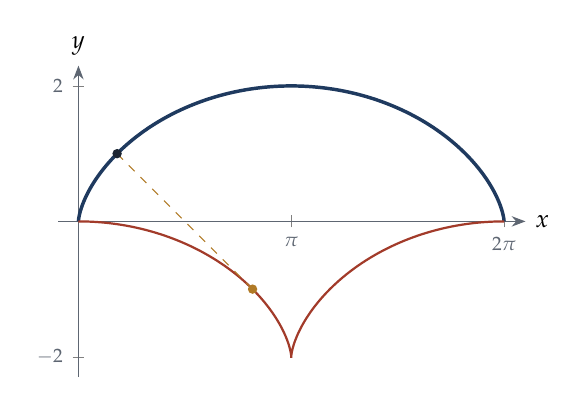
\begin{tikzpicture}
\begin{axis}[courbe,width=0.62\linewidth,xmin=-0.3,xmax=6.6,ymin=-2.3,ymax=2.3,xtick={3.1416,6.2832},xticklabels={$\pi$,$2\pi$},ytick={-2,2}]
\addplot[arcetude,domain=0:6.2832,samples=150]({x-sin(x)},{1-cos(x)});
\addplot[Brique,thick,domain=0:6.2832,samples=150]({x+sin(x)},{cos(x)-1});
\draw[Ocre,dashed] (axis cs:1.5708-1,1)--(axis cs:1.5708+1,-1);
\node[pt] at (axis cs:0.5708,1) {}; \node[pt,fill=Ocre] at (axis cs:2.5708,-1) {};
\end{axis}
\end{tikzpicture}
\end{center}
\retenir{la factorisation par l'angle moitié donne en même temps $v$, $\alpha$, $\ve T$, $\ve N$ ; la développée d'une cycloïde est
une cycloïde (propriété utilisée par Huygens pour le pendule isochrone).}
\end{corrige}

\subsection*{Chapitre 2 --- Enveloppes}
\addcontentsline{toc}{subsection}{Chapitre 2 --- Enveloppes}
\markboth{3\quad Corrigés --- Chapitre 2}{}
\begin{corrige}{e-segment}
\choix{la droite a une équation simple ; méthode~\ref{meth:enveloppe} : on résout le système formé de l'équation et de sa dérivée
par rapport à $t$.}
\q{1.} $\mathcal D_t:\frac xt+\frac y{1-t}=1$, soit $(1-t)x+ty=t-t^2$. En dérivant par rapport à $t$ : $-x+y=1-2t$. On reporte
$y=x+1-2t$ : $x+t-2t^2=t-t^2$, d'où $x=t^2$ et $y=(1-t)^2$. L'enveloppe est la courbe $t\mapsto\big(t^2,(1-t)^2\big)$.

\q{2.} $\sqrt x+\sqrt y=t+(1-t)=1$. En élevant au carré deux fois : $(1-x-y)^2=4xy$, soit $(x-y)^2-2(x+y)+1=0$. La partie
quadratique $(x-y)^2$ est un carré : c'est un arc de \emph{parabole}, d'axe $y=x$, tangent aux axes en $(1,0)$ et $(0,1)$.
\begin{center}
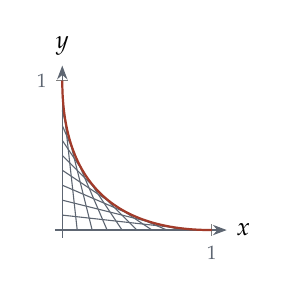
\begin{tikzpicture}
\begin{axis}[courbe,width=0.36\linewidth,xmin=-0.05,xmax=1.1,ymin=-0.05,ymax=1.1,xtick={1},ytick={1}]
\foreach \a in {0.1,0.2,0.3,0.4,0.5,0.6,0.7,0.8,0.9}{\edef\tmp{\noexpand\addplot[Gris,thin] coordinates {(\a,0) (0,{1-\a})};}\tmp}
\addplot[Brique,thick,domain=0:1,samples=60]({x^2},{(1-x)^2});
\end{axis}
\end{tikzpicture}
\end{center}
\piege{élever au carré introduit des points étrangers (la parabole entière contient aussi des points où
$\sqrt x-\sqrt y=\pm1$) : l'enveloppe n'est que l'arc $x,y\in[0,1]$.}
\retenir{droite d'équation $a(t)x+b(t)y=c(t)$ $\Rightarrow$ dériver par rapport au paramètre et résoudre le système $2\times2$.}
\end{corrige}
\begin{corrige}{e-ellipse}
\choix{théorème~\ref{thm:dev-env} : plutôt que de calculer $R$ et $\ve N$, on enveloppe les normales, ce qui ne demande qu'un
système linéaire.}
\q{1.} La normale passe par $M(t)$ et est orthogonale à $f'(t)=(-a\sin t,b\cos t)$ :
$-a\sin t\,(x-a\cos t)+b\cos t\,(y-b\sin t)=0$, soit
\[ax\sin t-by\cos t=(a^2-b^2)\sin t\cos t.\]
\q{2.} En dérivant par rapport à $t$ : $ax\cos t+by\sin t=(a^2-b^2)\cos2t$. Le système a pour déterminant
$ab(\sin^2t+\cos^2t)=ab\neq0$ ; on obtient
\[x=\frac{a^2-b^2}a\cos^3t,\qquad y=-\frac{a^2-b^2}b\sin^3t.\]
La développée est une astroïde étirée (astroïde de Lamé), avec quatre rebroussements sur les axes.

\q{3.} En $t=0$ : le centre de courbure est $\left(a-\frac{b^2}a,0\right)$, à la distance $\frac{b^2}a$ du sommet $(a,0)$ ; en $t=\frac\pi2$ :
$\left(0,b-\frac{a^2}b\right)$, à la distance $\frac{a^2}b$ de $(0,b)$. Ce sont bien les rayons de courbure trouvés.
\begin{center}
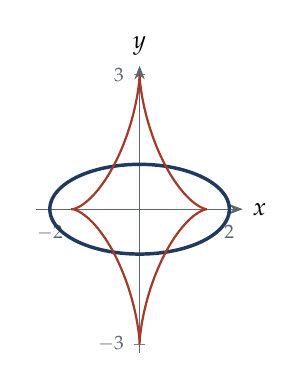
\begin{tikzpicture}
\begin{axis}[courbe,width=0.5\linewidth,xmin=-2.3,xmax=2.3,ymin=-3.2,ymax=3.2,xtick={-2,2},ytick={-3,3}]
\addplot[arcetude,domain=0:6.2832,samples=150]({2*cos(x)},{sin(x)});
\addplot[Brique,thick,domain=0:6.2832,samples=200]({1.5*cos(x)^3},{-3*sin(x)^3});
\end{axis}
\end{tikzpicture}
\end{center}
\gain{les quatre rebroussements de la développée correspondent aux quatre sommets de l'ellipse, où la courbure est
extrémale : c'est le réflexe du chapitre~1.}
\retenir{développée $=$ enveloppe des normales : équation de la normale, dérivée par rapport au paramètre, système $2\times2$.}
\end{corrige}
\clearpage
\ongletsfalse
\section*{Index des méthodes}\label{sec:index}
\addcontentsline{toc}{section}{Index des méthodes}
\markboth{Index des méthodes}{}
{\small\listemethodes}

\end{document}
